\chapter{Aan de slag}
\label{ch:aan-de-slag}

In dit hoofdstuk vind je wat technische achtergrond over een aantal onderwerpen die in de labo-opdrachten aan bod kunnen komen. Alles wat hier meegegeven wordt is gebaseerd op jarenlange ervaring, en typische problemen die studenten tegenkomen.

De bedoeling is om een minimum aan informatie mee te geven om je in staat te stellen snel aan de slag te gaan en een aantal typische beginnersfouten te vermijden. Voordat je aan de opdracht begint, lees je dus best eerst de informatie hier na en ga je ook best de \textbf{gerefereerde bronnen opzoeken en bestuderen}!

\section{Opzetten werkomgeving}
\label{sec:opzetten_werkomgeving}

Installeer eerst de nodige software, meer bepaald de laatste stabiele versie van de applicaties opgesomd in Sectie~\ref{ssec:software}. De volledige neerslag van al wat je voor deze cursus doet wordt bijgehouden in het versiebeheersysteem Git. Via Chamilo vind je een link die, als je er op doorklikt, een nieuwe repository creëert waar je in kan werken. Deze is zichtbaar voor jou en de lector. Naast de configuratie van de opgezette systemen zal je er ook je documentatie bijhouden, zoals testrapporten, procedures, cheat sheets en checklists.

Richtlijnen voor het opstarten van je Git project:

\begin{enumerate}
  \item In principe moet je al een Github account hebben. Als je dit nog niet gedaan hebt, koppel dan zeker je @student.hogent.be adres aan het account. Je kan dan het Github Student Developer Pack\footnote{\url{https://education.github.com/pack}} aanvragen met allerlei interessante aanbiedingen.
  \item Maak een SSH-sleutelpaar aan om het pushen naar Github te vereenvoudigen. Het commando is \texttt{ssh-keygen}, volg de richtlijnen die het geeft. Geef voor je gemak een lege \emph{passphrase} op (zoniet moet je telkens je de sleutel gebruikt je passphrase intikken). Normaal zou er in de directory \path{~/.ssh}\footnote{Het symbool {\textasciitilde} is natuurlijk de \emph{home directory} van de gebruiker. In Linux komt dit overeen met \path{/home/USER}, onder Windows met \path{C:\Users\USER} of \path{C:\Gebruikers\USER}, onder MacOS met \path{/Users/USER}} twee bestanden aangemaakt moeten zijn: \path{id_rsa} en \path{id_rsa.pub}. Het eerste is je private sleutel (die je geheim moet houden), het tweede de publieke. Die laatste kan je op Github registreren via je profielinstellingen (klik op je avatar rechtsboven, volg \emph{Settings} en dan \emph{SSH and GPG keys}).

  \item Basisconfiguratie Git, indien je dit nog niet gedaan hebt (kijk na in het configuratiebestand \path{~/.gitconfig}):

    \begin{minted}[gobble=6]{console}
      $ git config --global user.name "VOORNAAM NAAM"
      $ git config --global user.email "VOORNAAM.NAAM@student.hogent.be"
      $ git config --global push.default simple
      $ git config --global core.autocrlf input
      $ git config --global pull.rebase true
    \end{minted}

  \item Maak lokaal een directory aan die je voorbehoudt voor al wat met deze cursus te maken heeft. Binnen deze directory kan je je Github-repository klonen. Klik op de Github-pagina van je repository op de groene knop rechts (\emph{Clone or download}), kies voor ``Clone with SSH'' kopieer de link van de vorm \path{git@github.com:HoGentTIN/REPO_NAAM-GEBRUIKERSNAAM.git}.

    \begin{minted}[gobble=6]{console}
      $ cd Documents/Courses/EnterpriseLinux/
      $ git clone git@github.com:HoGentTIN/REPONAAM-GEBRUIKERSNAAM.git repo
    \end{minted}

  Dit maakt een lokale kopie van de repository in een subdirectory \path{repo}. Je kan zelf de naam van deze directory kiezen en die achteraf verplaatsen, alles blijft gewoon werken.
  
  \item Creëer een nieuwe \emph{branch} met de naam \texttt{solution} om je eigen code en documentatie bij te houden. Verderop wordt duidelijk waarom dit belangrijk is.

    \begin{minted}[gobble=6,linenos=false]{console}
      $ git checkout -b solution
    \end{minted}

  \item Bekijk de bestanden in de \path{assignment/} directory. Hier vind je de opgave van deelopdrachten en sjablonen voor verslagen en cheat sheets in Markdown-formaat~\autocite{Gruber2004}. Pas alvast het sjabloon aan, vul er je eigen naam in.
\end{enumerate}

Wanneer er errata in de opgave gepubliceerd worden, kan je die relatief eenvoudig binnen halen, maar enkel als je een eigen branch aangemaakt hebt.

\begin{enumerate}
  \item Eerst moet je zorgen dat je updates kan binnenhalen van de repository met de opdracht. Het volgende commando zorgt dat je kan synchroniseren met die repository. Dit moet slechts één keer gebeuren.

    \begin{minted}[gobble=6,linenos=false]{console}
      $ git remote add upstream https://github.com/HoGentTIN/elnx-sme.git
    \end{minted}

  \item Wanneer er nieuwe commits gebeurd zijn in de opgave, kan je de wijzigingen telkens zo ophalen:

    \begin{minted}[gobble=6]{console}
      $ git checkout master
      $ git pull upstream master
      $ git checkout solution
      $ git rebase master
    \end{minted}

    \begin{itemize}
      \item De eerste twee regels zorgen er voor dat jouw versie van de master-branch up-to-date gebracht wordt met de nieuwe commits.
      \item In de derde regel ga je opnieuw naar je eigen branch. Voorlopig is er daar nog niets gewijzigd
      \item In de vierde regel, tenslotte, ga je de wijzigingen in de opgave op jouw eigen versie toepassen. Mogelijks komen er hier conflicten naar boven tussen bepaalde bestanden in de opgave en jouw wijzigingen. Lees goed de instructies die Git hier geeft om deze conflicten op te lossen.
    \end{itemize}

Deze procedure werkt niet als je geen branch voor je eigen oplossing gemaakt hebt. In dat geval haal je jezelf een hoop ellende op de hals\ldots

\end{enumerate}

\section{Algemene richtlijnen}
\label{sec:algemene_richtlijnen}

In deze sectie vind je enkele algemene richtlijnen die je helpen vlotter en efficiënter te werken.

\begin{itemize}
  \item Voor je aan een (deel-)opdracht begint, bereid je eerst voor door alle aangereikte studiematerialen te bestuderen: handleidingen, screencasts, \ldots Die ``van buiten blokken'' is helemaal niet nodig, maar zorg er in elk geval voor dat je er in die mate vertrouwd bent, dat je snel gericht kan zoeken naar juiste, relevante informatie. Je vindt die via de bronvermeldingen in deze syllabus, of via de opgave
  \item Open \textbf{verschillende terminalvensters/consoles naast elkaar} (zie Figuur~\ref{fig:screenshot-terminals}). Elke terminal krijgt zijn eigen functie, bijvoorbeeld:
    \begin{itemize}
      \item Vim editor (of VS Code/Sublime/Notepad/\ldots in een apart venster);
      \item doorvoeren van wijzigingen aan de configuratie;
      \item ingelogd op VM, voor commando's;
      \item ingelogd op VM, voor tonen logbestanden.
    \end{itemize}
  \item \textbf{Werk stap voor stap.} Schrijf niet teveel code ineens. Probeer eerst een minimaal werkende opstelling te verkrijgen en registreer meteen in Git. Maak minimale wijzigingen en \textbf{test elke wijziging uit}. Hoe groter en ingrijpender de wijzigingen, hoe meer kans op fouten en hoe moeilijker die te debuggen zijn. Zodra iets werkt, en je bent een stap verder, registreer je dit meteen in Git en geef je een duidelijke, beschrijvende commit-boodschap.
  \item \textbf{gebruik Git op de command-line.} Bij de meeste Git commando's krijg je gedetailleerde uitleg over hoe je een stap verder moet gaan en ook hoe je de laatste stap kan ongedaan maken. Dit geeft op de duur een beter inzicht in hoe Git precies werkt.
  \item Probeer \textbf{elke commit te beperken tot één enkele ``reden''} om wijzigingen aan te brengen aan de bestaande code. Dit maakt de ``geschiedenis'' van je project transparanter en maakt ook dat je makkelijker kan terugkeren naar een bepaalde stap wanneer je de mist in gaat.
  \item \textbf{Maak backups} van de originele, ongewijzigde configuratiebestanden zodat je er op kan terugvallen als er iets misloopt. Soms heb je zodanig zitten ``prutsen'' dat je er niet meer in slaagt de service te laten werken.
  \item \textbf{Gebruik \texttt{vagrant destroy}} (zie Sectie~\ref{sec:vagrant}). Wanneer je veel manuele wijzigingen hebt aangebracht in een VM, ben je op de duur niet meer zeker dat die zich in de gewenste toestand bevindt. Of je kan door experimenteren de VM onbruikbaar gemaakt hebben. Door de VM te verwijderen en opnieuw op te bouwen (met \texttt{vagrant up}) kan je opnieuw beginnen van een werkende versie (als je de vorige richtlijnen opvolgt, tenminste!).
  \item Ook wanneer je denkt klaar te zijn met een deelopdracht, genereer de VM nog eens helemaal opnieuw en voer alle acceptatietests uit.
\end{itemize}

\begin{figure}
  \centering
  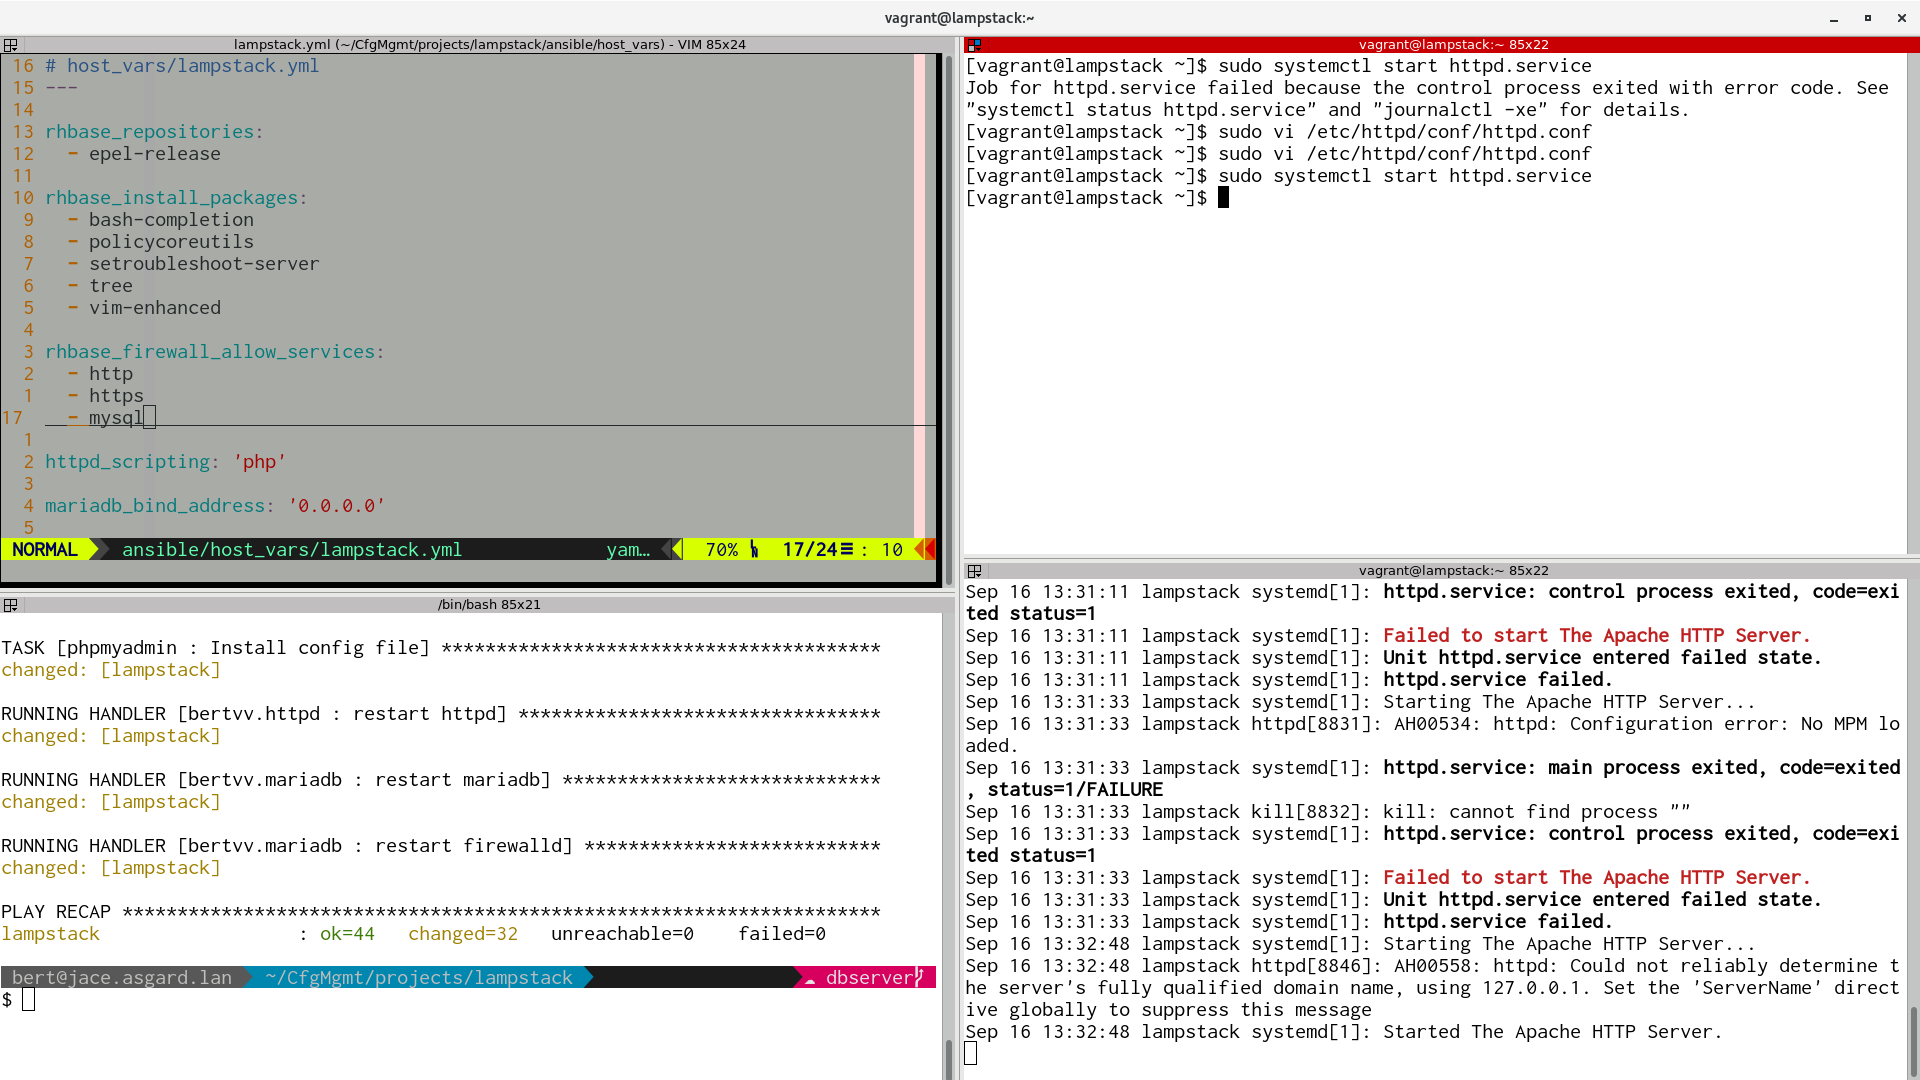
\includegraphics[width=\linewidth]{img/screenshot-terminals}
  \caption[Gebruik van verschillende terminals.]{\textbf{Gebruik van verschillende terminals.} In deze schermafbeelding is Terminator (een terminal-applicatie voor Linux) opgedeeld in vier aparte shells. Linksboven is Vim geopend met een broncodebestand. De terminal linksonder wordt gebruikt om wijzigingen in de broncode door te voeren op de virtuele machines. Rechtsboven is er ingelogd op de virtuele machine waar momenteel wijzigingen op aangebracht worden en kunnen commando's uitgevoerd worden om zaken uit te proberen of problemen op te sporen. Rechtsonder, tenslotte, worden relevante logbestanden van de VM getoond.}
  \label{fig:screenshot-terminals}
\end{figure}

\section{Bash tips}
\label{sec:bash_tips}

In deze sectie vind je een aantal tips voor het gebruik van de Bash-shell. In deze cursus maak je intensief gebruik van de shell, en het loont de moeite om Bash wat beter te leren kennen. Het zit immers vol met interessante features die je toelaten productiever te werken. Online is hier nog veel meer over te vinden~\autocite{Rowe2009}.

De tips hier gelden ook voor Windows- en MacOS-gebruikers! Windows-gebruikers hebben beschikking over een recente versie van Bash via Git (Git Bash). In MacOS X zit ook een Bash-shell, weliswaar een zeer oude versie\footnote{Dit is omwille van de softwarelicentie. Recente versies van Bash vallen onder de open source GPL-licentie, waar Apple niets mee te maken wil hebben.}. Je kan een recente versie installeren via HomeBrew\footnote{\url{http://brew.sh}}.

\begin{itemize}
  \item \textbf{Gebruik \emph{\texttt{TAB}-completion}.} Je kan een deel van een commando of pad intikken en dan de \texttt{TAB}-toets indrukken. Indien mogelijk zal Bash het woord vervolledigen, of mogelijke alternatieven tonen. Als je de package \texttt{bash-completion} installeert zijn er nog veel meer mogelijkheden.
  \item \textbf{Gebruik de \emph{command history}.} Bash houdt de commando's die je eerder gebruikt hebt bij. Met de pijltjestoetsen kan je eerdere commando's terug halen. Gebruik \texttt{Ctrl-R} om te zoeken in de command history. Je kan dan een fragment van het commando intikken, Bash toont dan het laatste commando waar dat tekstfragment in voorkomt.
  \item \textbf{Bang bang!} In Bash zijn er enkele shortcuts voorzien voor (delen van) het vorige commando. \texttt{!!} staat voor het gehele vorige commando, \texttt{!\$} voor het laatste argument en \texttt{!*} voor alle argumenten. Een voorbeeldje van het gebruik:

    \begin{minted}{console}
$ yum update
You need to be root to perform this command.
$ sudo !!
sudo yum update
[...]
$ mkdir -p some/long/path/i/dont/want/to/repeat
$ cd !$
cd some/long/path/i/dont/want/to/repeat
$
\end{minted}
  \item \textbf{Toetsenbordcombinaties.} Naast \texttt{Ctrl-R} van hierboven zijn er nog een aantal nuttige toetsenbordcombinaties.
    \begin{itemize}
      \item \texttt{Ctrl-C} onderbreekt het huidige proces
      \item \texttt{Ctrl-Z} pauzeert het huidige proces (haal het terug met \texttt{fg})
      \item \texttt{Ctrl-D} sluit de shell af (enkel op lege regel)
      \item \texttt{Ctrl-K} verwijdert de tekst rechts van de cursor
      \item \texttt{Ctrl-U} verwijdert de tekst links van de cursor
      \item \texttt{Ctrl-T} verwisselt letterteken onder de cursor met dat voor de cursor
      \item \texttt{Alt-T} verwisselt woord voor met woord na de cursor
    \end{itemize}

    Er bestaan nog \emph{veel} meer combinaties. Deze kan je vinden in de man-pagina \texttt{bash(1)} in de sectie READLINE (subsectie \emph{Readline Command Names} en volgende).

  \item \textbf{Personaliseer de shell.} Je kan het gedrag van de shell in hoge mate aan je eigen wensen aanpassen door het bestand \path{~/.bashrc} aan te passen. Je kan het gedrag van tab-completion of de command history aanpassen, een eigen commandoprompt instellen, aliassen (zie verder) of functies definiëren, enz. Het zou ons te ver leiden om alle mogelijkheden uit te diepen, maar je kan een relatief eenvoudig voorbeeld vinden in \url{https://github.com/bertvv/server-dotfiles/} (installatie-instructies te vinden in de README), en een meer uitgebreid voorbeeld in \url{https://github.com/bertvv/dotfiles/} (of gelijknamige repositories van andere Github-gebruikers).

  \item \textbf{Aliassen} zijn een soort shortcuts voor commando's die je vaak gebruikt. Dit kan enorm veel typwerk besparen. Je kan ze toevoegen in je \path{~/.bashrc}. Enkele voorbeelden ter inspiratie:

    \begin{minted}{bash}
alias l='ls -l --si --time-style=long-iso --color'
alias a='git add'
alias c='git commit -m'
alias h='git log --pretty="format:%C(yellow)%h %C(blue)%ad %C(reset)%sC(red)%d %C(green)%an%C(reset), %C(cyan)%ar" --date=short --graph --all'
alias s='git status'
alias vu='vagrant up'
alias vD='vagrant destroy'
alias elnx='cd /home/bert/Documents/Courses/EnterpriseLinux/16-17'
\end{minted}

    Nog meer voorbeelden vind je in \url{https://github.com/bertvv/dotfiles/blob/master/.bash.d/aliases.sh}.
\end{itemize}

\section{Vagrant}
\label{sec:vagrant}

Vagrant is een command line tool die het aanmaken en configureren van virtuele machines automatiseert. Het ondersteunt een aantal virtualisatieplatforms, o.a.~VirtualBox, Hyper-V, libvirt, enz. Wij zullen het gebruiken in combinatie met VirtualBox. Voor een demo van de werking van Vagrant, bekijk eerst de screencast van \textcite{Weissig2014}.

Je Git repository bevat een Vagrant-omgeving voor het opzetten van de VMs voor je labo-opdracht. Er zijn alvast twee VMs gedefinieerd.  Je kan een overzicht van de VMs opvragen met (voorbeeld uit de SME-opdracht van Sectie~\ref{subs:smallmedium-enterprise-infrastructure}):

\begin{minted}{console}
$ vagrant status
Current machine states:

router                    not created (virtualbox)
pu001                     not created (virtualbox)

The environment has not yet been created. Run `vagrant up` to
create the environment. If a machine is not created, only the
default provider will be shown. So if a provider is not listed,
then the machine is not created for that environment.
$
\end{minted}

De initiële setup bevat twee virtuele machines met namen \texttt{router} en \texttt{pu001}, respectievelijk. We beginnen met \texttt{pu001}, de router wordt later geconfigureerd.

Start de VM met \texttt{vagrant\ up\ pu001}. De eerste keer dat je dit doet wordt er een basis-VM gedownload met een minimale installatie van de laatste stabiele versie van CentOS. Doe dit best op een performant netwerk: het bekabelde netwerk op de campus of thuis/op kot. Deze ``base box'' wordt bijgehouden en zal telkens dienst doen als basis voor het opzetten van alle hosts in ons netwerk. Het downloaden gebeurt dus slechts één keer-.

Na opstarten kan je inloggen met \texttt{vagrant\ ssh\ pu001}. Je bent ingelogd als gebruiker \texttt{vagrant} en kan commando's uitvoeren met \texttt{root}-rechten door er \texttt{sudo} voor te plaatsen (geen wachtwoord vereist). Als het nodig mocht zijn: het wachtwoord van de gebruikers \texttt{vagrant} en \texttt{root} is telkens \texttt{vagrant}.

Als je \texttt{ls\ /} uitvoert, zal je merken dat er een directory \path{/vagrant} bestaat. Dit is je lokale repository die gemount is binnen de VM. Dit is een eenvoudige manier om bestanden te delen tussen VM en host-systeem.

Let er op dat je VMs niet meer vanuit je VirtualBox GUI opstart of bewerkt. Doe dit nu enkel met Vagrant en vanuit een terminal. Het commando \texttt{vagrant} moet altijd uitgevoerd worden vanuit de directory waar het bestand \texttt{Vagrantfile} zich bevindt.

De belangrijkste Vagrant commando's worden opgesomd in Tabel~\ref{tab:vagrant-commandos}. Daar waar \texttt{[VM]} tussen rechte haken staat, is dat een optioneel argument. Als je het weglaat, wordt de actie op \emph{alle} VMs tegelijk uitgevoerd.

\begin{longtable}{@{}ll@{}}
  \toprule
  Commando & Functie\tabularnewline
  \midrule
  \endhead
  \texttt{vagrant\ status} & Geef een overzicht van de Vagrant-omgeving\tabularnewline
  \texttt{vagrant\ up\ [VM]} & Start \texttt{VM} op\tabularnewline
  \texttt{vagrant\ provision\ [VM]} & Draai het configuratiescript op \texttt{VM}\tabularnewline
  \texttt{vagrant\ ssh\ VM} & Log in op \texttt{VM} als gebruiker \texttt{vagrant}\tabularnewline
  \texttt{vagrant\ halt\ [VM]} & Stop \texttt{VM}\tabularnewline
  \texttt{vagrant\ reload\ [VM]} & Herstart \texttt{VM}\tabularnewline
  \texttt{vagrant\ destroy\ [VM]} & Vernietig \texttt{VM}\tabularnewline
  \bottomrule
\caption{De belangrijkste \texttt{vagrant}-commando's}
\label{tab:vagrant-commandos}
\end{longtable}

Alle VMs in de opstelling krijgen twee netwerkinterfaces:

\begin{itemize}
  \item Adapter 1: NAT-interface (de ``management interface'' voor Vagrant, Internetverbinding voor de VM)
  \item Adapter 2: Host-only interface (gebruikt om vanop het hostsysteem de netwerkservices op de VM aan te spreken)
\end{itemize}

Zorg dat je goed begrijpt hoe deze interfaces werken, zoniet wordt troubleshooten erg moeilijk~\autocite{VanVreckem2015a}.

\section{Ansible}
\label{sec:ansible}

Ansible is een \emph{configuration management system,} d.w.z. het staat in voor het configureren van een host vanaf een minimale installatie tot een volledig operationeel systeem. Het concept van een configuration management tool is dat je beschrijft wat de gewenste toestand van het systeem is, de tool brengt het systeem naar die toestand. Bekijk de screencast van \textcite{Weissig2015} voor een inleiding op Ansible. In een vervolg-screencast wordt ook de combinatie van Ansible en Vagrant belicht. In deze gids geven we enkel wat uitleg om aan de slag te gaan met de startopstelling voor de labo-opdracht, maar als je op zoek bent naar een goed naslagwerk over Ansible, overweeg dan om het e-boek van \textcite{Geerling2016} te kopen. Het boek is al enkele jaren oud, maar de auteur werkt nog verder aan het boek, updates zijn gratis.

Sommige config management systemen hebben een eigen taal ontwikkeld om die configuratie in te beschrijven (bv. Puppet), andere gebruiken een bestaande taal (bv. Chef, configuratie in Ruby). Bij Ansible beschrijf je de configuratie van een systeem met YAML (een variant van JSON), een eenvoudig tekstformaat om data te structureren op een manier die makkelijk te interpreteren is zowel door mensen als computers. De bestanden die deze configuratiecode bevatten worden \emph{playbooks}\footnote{\url{https://docs.ansible.com/ansible/playbooks.html}} genoemd. Als je deze playbooks op een specifieke manier structureert en herbruikbaar maakt, spreekt men van een \emph{rol}\footnote{\url{https://docs.ansible.com/ansible/playbooks_roles.html\#roles}}. Je kan rollen toekennen aan een host, en specifieke instellingen toepassen door het invullen van \emph{variabelen}\footnote{\url{https://docs.ansible.com/ansible/playbooks_variables.html}}. Op Ansible Galaxy\footnote{\url{https://galaxy.ansible.com/}} kan je tientallen rollen vinden die door hun auteurs gepubliceerd zijn.

De directorystructuur van een Ansible-project ligt vast en wordt uitvoerig beschreven in de documentatie\footnote{\url{https://docs.ansible.com/ansible/playbooks_best_practices.html}}.

\subsection{Rollen toekennen aan hosts}
\label{sub:rollen-toekennen-aan-hosts}

Om een rol toe te kennen aan een host, bewerk je de \emph{master playbook} \path{ansible/site.yml}. Dit bestand bevat een overzicht van alle hosts onder het beheer van Ansible, met de rollen van elke host (spaties worden getoond):

\begin{minted}[showspaces]{yaml}
# site.yml
---
- hosts: pu001
  become: true
  roles: []
\end{minted}

Host \texttt{pu001} heeft nog geen rollen toegekend, dat gaan we nu veranderen:

\begin{minted}[showspaces]{yaml}
# site.yml
---
- hosts: pu004
  become: true
  roles:
    - bertvv.rh-base
\end{minted}

Onder \texttt{roles:} kan je zoveel rollen toevoegen als nodig. Let goed op de indentatie. Je \textbf{moet} telkens inspringen met 2 spaties, en alle data op hetzelfde niveau moet links mooi uitgelijnd zijn.

\subsection{Rollen installeren}
\label{sub:rollen-installeren}

Alle rollen die gebruikt worden in \path{site.yml} moeten beschikbaar zijn in de directory \path{ansible/roles/} in een subdirectory met dezelfde naam als deze gebruikt in \path{site.yml}.

De naam van de rol \path{bertvv.rh-base} is geschreven in de vorm \path{AUTEUR.ROLNAAM}. Dit wijst er op dat deze rol op Ansible Galaxy gepubliceerd is. Je kan die daar terugvinden onder de url ``\url{http://galaxy.ansible.com/AUTEUR/ROLNAAM/}.'' Je kan daar de rol downloaden en uitpakken op de juiste plaats in de Ansible-directorystructuur.

Dit is het eenvoudigste als je \textbf{MacOS of Linux} op je hostsysteem draait. Je kan dan Ansible installeren en gebruik maken van het commando \texttt{ansible-galaxy}:

\begin{minted}{console}
$ ansible-galaxy -p ansible/roles install bertvv.httpd
- downloading role 'httpd', owned by bertvv
- downloading role from https://github.com/bertvv/ansible-role-httpd/archive/v1.2.1.tar.gz
- extracting bertvv.httpd to ansible/roles/bertvv.httpd
- bertvv.httpd was installed successfully
$
\end{minted}

Dit commando zal de rol \path{bertvv.rh-base} downloaden en uitpakken onder directory \path{ansible/roles}.

Onder \textbf{Windows} wordt Ansible niet ondersteund, en is dit commando dus ook niet beschikbaar. Je kan wel manueel een rol downloaden van de Github-repository (bijvoorbeeld voor \path{bertvv.rh-base} van \url{https://github.com/bertvv/ansible-role-rh-base/releases}) en dan op de juiste plaats uitpakken.

In je repository is ook een scriptje voorzien dat het installatieproces automatiseert: \path{scripts/role-deps.sh}. Als je het uitvoert in een Bash shell vanuit de hoofddirectory van je repository, zal het in \path{ansible/site.yml} alle rollen die er vernoemd worden van Ansible Galaxy (of indien de rol daar niet gepubliceerd is van Github) downloaden en installeren. Dit script werkt trouwens ook op MacOS en Linux.

\begin{minted}{console}
$ ./scripts/role-deps.sh 
- downloading role 'rh-base', owned by bertvv
- downloading role from https://github.com/bertvv/ansible-role-rh-base/archive/v2.3.0.tar.gz
- extracting bertvv.rh-base to /home/bert/Documents/Vakken/enterprise-linux/opgaven/elnx-sme-bertvv/ansible/roles/bertvv.rh-base
- bertvv.rh-base (v2.3.0) was installed successfully
$ 
\end{minted}

Merk op dat rollen van Ansible Galaxy genegeerd worden door Git. Het heeft geen zin je eigen repository te ``vervuilen'' met code die al elders onderhouden wordt. Het is dus ook de bedoeling dat je \emph{geen wijzigingen} aanbrengt in bestaande rollen. Als dit toch nodig is (omdat er bv. features ontbreken die je zelf geïmplementeerd hebt), is het beter de oorspronkelijke rol te ``forken'' op Github en daar te onderhouden.

Na installatie van de rollen, kan je met \texttt{vagrant\ provision} de \emph{master playbook} uitvoeren.

\subsection{Hosts configureren}
\label{sub:hosts-configureren}

Als je de documentatie voor een rol naleest (typisch het bestand README.md van de Github repository), vind je in principe een lijst met \emph{rolvariabelen} die je kan invullen voor het toepassen van concrete instellingen voor hetzij specifieke hosts, hetzij groepen van hosts. Variabelen die voor \emph{alle} hosts gelden, moeten gedefinieerd worden in het bestand \path{ansible/group_vars/all.yml}. Variabelen voor specifieke hosts in \path{ansible/host_vars/HOSTNAAM.yml}. Het formaat is opnieuw Yaml, en de structuur van zo'n bestand is zeer eenvoudig. Je geeft een opsomming van variabelen met de waarde die je er aan wil geven. Een voorbeeld:

\begin{minted}{yaml}
---
rhbase_repositories:
  - epel-release
rhbase_install_packages:
  - bash-completion
  - vim-enhanced
rhbase_firewall_allow_services
  - http
  - https
\end{minted}

Telkens je een wijziging aanbrengt in de Ansible-configuratie, kan je die doorvoeren met \texttt{vagrant\ provision}. Het is dan normaal niet nodig om de VM te rebooten of te verwijderen en opnieuw op te zetten.

\section{Basiskennis CentOS}
\label{sec:basiskennis_centos}

CentOS is een Linux-distributie die afgeleid is van RedHat, maar initieel volledig door de \emph{community} onderhouden werd. RedHat is een commerciële Linux-dis\-tri\-bu\-tie van het gelijknamige bedrijf. Je kan RedHat Enterprise Linux (RHEL) enkel gebruiken als je er een support contract voor tekent. Nu is RHEL wel volledig open source en is het dus toegelaten om de code te hergebruiken en te wijzigen. Dat is precies wat in het CentOS-project gebeurd is. Alles wat onder het merkenrecht valt (de naam RHEL, logo's, enz.) is verwijderd en vervangen. CentOS is dus volledig compatibel met RHEL, maar gratis, zij het zonder support vanuit RedHat. RedHat heeft echter wel goede relaties met het CentOS-project, zelfs in die mate dat ze sinds 2014 het project beginnen sponsoren zijn en de belangrijkste medewerkers van het project in dienst genomen hebben. In deze cursus gebruiken we CentOS omdat de RedHat-familie in het Vlaamse bedrijfsleven de meest gebruikte Linux-dis\-tri\-bu\-tie is.

Om je te helpen bij het leren kennen van deze distributie vind je hieronder enkele suggesties.

\begin{itemize}
  \item \textbf{Lees eerst de RHEL 7-documentatie}~\autocite{SvistunovEtAl2016,JahodaEtAl2016,JahodaEtAl2016a}, ga niet in het wilde weg Googlen naar commando's. Recent zijn er redelijk wat ingrijpende wijzigingen gebeurd in het Linux-landschap waardoor vele commando's die nog altijd in blog-artikels en HOWTO's staan niet meer werken of verouderd zijn. De delen van de handleidingen die bij uitstek relevant zijn, worden opgesomd in Sectie~\ref{sec:leerdoelen}.
  \item Maak voor jezelf een \textbf{cheat sheet} met de belangrijkste commando's, in het bijzonder voor:
    \begin{itemize}
      \item netwerkinstellingen opvragen met \texttt{ip};
      \item de werking van \texttt{sudo};
      \item installatie van software beheren met \texttt{yum};
      \item services beheren met \texttt{systemctl};
      \item de firewall beheren met \texttt{firewall-cmd};
      \item de juiste commando's voor het valideren van configuratiebestanden, bv.
      \begin{itemize}
        \item Samba: \texttt{testparm}
        \item Apache: \texttt{apachectl configtest}
        \item BIND: \texttt{named-checkconf}
        \item ISC-dhcpd: \texttt{dhcpd -t}
        \item \ldots
      \end{itemize}
    \end{itemize}

    Je kan je laten inspireren door deze cheat sheet: \url{https://github.com/bertvv/cheat-sheets/blob/master/src/EL7.md} Kopieer deze niet blind! Je moet je eigen cheat sheet zelf opstellen, zo zal je de commando's beter onthouden.
\end{itemize}

\section{DNS en BIND}
\label{sec:dns-en-bind}

DNS is essentieel voor de correcte werking van een domein, en redelijk wat (volgens sommigen \emph{alle}\footnote{\url{http://www.krisbuytaert.be/blog/}}) netwerkproblemen zijn terug te leiden tot fouten in DNS. Er zijn verschillende implementaties van DNS, maar veruit de meest gebruikte (en dus essentieel voor de werking van het Internet als geheel) is BIND\footnote{\url{https://www.isc.org/downloads/bind/}}.

In deze syllabus geven we een heel summiere inleiding. Voor een uitgebreid overzicht van de werking en configuratie van BIND, zie~\textcite{Aitchison2015}.

\subsection{Zonebestanden}
\label{ssec:zonebestanden}

DNS is op zich geen complexe netwerkservice. Het komt neer op een databank met enkele tabellen (= zonebestanden) die in (een strak) tekstformaat zijn opgemaakt. Er zijn verschillende types van records, o.a.

\begin{itemize}
\item \texttt{A} bevat het IPv4-adres voor een gegeven hostnaam;
\item \texttt{AAAA} idem, maar voor IPv6;
\item \texttt{CNAME} bevat de ``originele'' hostnaam voor een gegeven alias (kan bijvoorbeeld worden gebruikt voor ``www.linuxlab.lan'');
\item \texttt{MX} bevat verwijzingen naar de mailservers voor dit domein;
\item \texttt{NS} bevat verwijzingen naar de DNS-servers voor dit domein;
\item \texttt{PTR} bevat de hostnaam voor een gegeven IP-adres (bevindt zich normaal in een zgn.\emph{reverse lookup} zonebestand);
\item enz. (lees de documentatie!)
\end{itemize}

Een zonebestand begint met een zgn. SOA-record, wat staat voor Start Of Authority. Hieronder vind je een voorbeeld van een \emph{forward zone file} voor een domein met de naam ``linuxlab.lan'' voor het IPv4-netwerk 192.168.15.0/24. Op de precieze betekenis gaan we hier niet in, dit wordt elders voldoende uitgediept~\autocite{Aitchison2015}.

\begin{minted}{text}
; /var/named/linuxlab.lan
; Forward lookup zone file for `linuxlab.lan.'
$ORIGIN linuxlab.lan.
$TTL 1W
;        primary DNS   email address admin
@ IN SOA srv001        hostmaster (
   2015101216   ; serial
   1D           ; refresh
   1H           ; retry
   1W           ; expire
   1D           ; minimum TTL
)
\end{minted}

De overeenkomstige \emph{reverse zone file} begint als volgt:

\begin{minted}{text}
; /var/named/15.168.192.in-addr.arpa.
; Reverse lookup zone file for `linuxlab.lan.'
$ORIGIN 15.168.192.in-addr.arpa.
$TTL 1W
@ IN SOA srv001.linuxlab.lan. hostmaster.linuxlab.lan. (
   2015101216   ; serial
   1D           ; refresh
   1H           ; retry
   1W           ; expire
   1D           ; minimum TTL
)
\end{minted}

De syntax van deze \emph{zone files} is heel strak en het is makkelijk om fouten te maken. De meest voorkomende fouten zijn de volgende:

\begin{itemize}
  \item Hostnamen die volledig uitgeschreven zijn (\emph{fully qualified domain name} of FQDN) moeten in een zonebestand altijd afgesloten worden met een punt, bv. ``\texttt{pu001.linuxlab.lan.}''. Namen die niet op een punt eindigen, worden aangevuld met de waarde van \texttt{\$ORIGIN} die aan het begin van een zonebestand gegeven wordt (d.i. de domeinnaam, in ons geval ``\texttt{linuxlab.lan.}''). Bv.  \texttt{pu002} wordt dan ``\texttt{pu002.linuxlab.lan.}''. Als je een hostnaam volledig uitschrijft en je vergeet de punt, dan zal de domeinnaam dus verkeerd geïnterpreteerd worden. ``\texttt{pu002.linuxlab.lan}'' wordt immers omgezet naar ``\path{pu002.linuxlab.lan.linuxlab.lan.}''.
  
  \item IP-adressen worden op een eigenaardige manier genoteerd. Ten eerste wordt het host-deel van het netwerkadres niet geschreven, de getallen in de ``dotted quad''-notatie worden omgekeerd en je moet er ``\texttt{in-addr.arpa.}'' achter schrijven. Met andere woorden, \texttt{192.0.2.0/24} wordt als ``\texttt{2.0.192.in-addr-arpa."} geschreven.
\end{itemize}

\subsection{DNS troubleshooting}
\label{ssec:dns-troubleshooting}

Het is niet altijd evident om fouten op te sporen in de configuratie van een BIND DNS-server. Daarom deze tips:

\begin{itemize}
  \item Test de syntax van configuratiebestanden voordat je de service opstart. Voor het hoofd-configuratiebestand \path{/etc/named.conf} is het commando:
    \begin{minted}[gobble=6,linenos=false]{console}
      $ sudo named-checkconf /etc/named.conf
    \end{minted}
  \item De syntax testen van zonebestanden gebeurt zo (voorbeeld voor forward en reverse zone, respectievelijk):

    \begin{minted}[gobble=6]{console}
      $ sudo named-checkzone linuxlab.lan /var/named/linuxlab.lan
      $ sudo named-checkzone 15.168.192.in-addr.arpa \
          /var/named/15.168.192.in-addr.arpa
    \end{minted}

\item Je kan foutboodschappen van de service bekijken met \texttt{journalctl}. Het handigste is om een aparte console te openen, in te loggen op je server en dan het volgende commando uit te voeren:

    \begin{minted}[gobble=6]{console}
      $ sudo rndc querylog on
      $ sudo journalctl -l -f -u named.service
    \end{minted}

  Het eerste commando zorgt dat DNS-queries van clients in de logs verschijnen (wat standaard uit staat). Het tweede commando toont de logs van BIND.

  Open een andere console om commando's uit te voeren (bv. de service herstarten). Je ziet dan meteen relevante info- en foutboodschappen verschijnen.
\end{itemize}

Naast het valideren van de configuratiebestanden, is het ook belangrijk om te testen of de DNS-server ook correct antwoordt op aanvragen van clients. Installeer de package \texttt{bind-tools} om een aantal nuttige tools ter beschikking te krijgen. Het commando \texttt{nslookup} zal je misschien herkennen vanuit Windows. Het werkt hier op dezelfde manier:

\begin{minted}{console}
$ nslookup www.hogent.be
Server:   195.130.131.1
Address:  195.130.131.1\#53

Non-authoritative answer:
Name:  www.hogent.be
Address: 178.62.144.90
\end{minted}

Hier wordt gevraagd wat het IP-adres is voor hostnaam ``www.hogent.be''. Als antwoord krijgen we 178.62.144.90. Het antwoord werd gegeven door een DNS-server met IP-adres 195.130.131.1. Er wordt aangegeven dat het antwoord \emph{non-authoritative} is, wat wil zeggen dat de DNS-server die het antwoord gaf niet de DNS-server is die ook de eindverantwoordelijke is voor het hogent.be-domein.

Je kan een query met \texttt{nslookup} ook richten naar een specifieke DNS-server door die ook mee te geven op de command line:

\begin{minted}{console}
$ nslookup www.hogent.be 8.8.8.8
Server:		8.8.8.8
Address:	8.8.8.8#53

Non-authoritative answer:
Name:	www.hogent.be
Address: 178.62.144.90
\end{minted}

Merk op dat als je de DNS-server niet expliciet vermeldt, de DNS-server ondervraagd wordt die door DHCP werd toegewezen en die vermeld wordt in het bestand \texttt{/etc/resolv.conf}.

Naast \texttt{nslookup}, bevat de \texttt{bind-utils} een nog veelzijdiger commando om DNS-servers te ondervragen: \texttt{dig}.

\begin{minted}{console}
$ dig www.hogent.be

; <<>> DiG 9.10.5-P2-RedHat-9.10.5-2.P2.fc25 <<>> www.hogent.be
;; global options: +cmd
;; Got answer:
;; ->>HEADER<<- opcode: QUERY, status: NOERROR, id: 23001
;; flags: qr rd ra; QUERY: 1, ANSWER: 1, AUTHORITY: 0, ADDITIONAL: 1

;; OPT PSEUDOSECTION:
; EDNS: version: 0, flags:; udp: 4096
;; QUESTION SECTION:
;www.hogent.be.			IN	A

;; ANSWER SECTION:
www.hogent.be.		2796	IN	A	178.62.144.90

;; Query time: 11 msec
;; SERVER: 195.130.131.1#53(195.130.131.1)
;; WHEN: Tue Sep 26 00:45:51 CEST 2017
;; MSG SIZE  rcvd: 58
\end{minted}

De syntax van de uitvoer is compatibel met die van zonebestanden. We zien hier dus dat er voor www.hogent.be een A-record bestaat dat verwijst naar IP-adres 178.62.144.90. Alle regels die beginnen met een kommapunt zijn commentaar.

Je kan vragen enkel de relevante info af te drukken, zonder de commentaren:

\begin{minted}{console}
$ dig +short www.hogent.be
178.62.144.90
\end{minted}

Een specifieke DNS-server ondervragen gebeurt door die op de command-line mee te geven, voorafgegaan door een ``@'':

\begin{minted}{console}
$ dig +short @8.8.8.8 www.hogent.be
178.62.144.90
\end{minted}

Tenslotte kan je ook verschillende soorten records opvragen. Bijvoorbeeld, wie is de ``authoritative name server'' voor het domein hogent.be?

\begin{minted}{console}
$ dig +short NS hogent.be
ns2.belnet.be.
ens2.hogent.be.
ns1.belnet.be.
ens1.hogent.be.
\end{minted}

Wat is het IPv6 adres voor download.fedoraproject.org?

\begin{minted}{console}
$ dig +short AAAA download.fedoraproject.org
wildcard.fedoraproject.org.
2001:4178:2:1269::fed2
2610:28:3090:3001:dead:beef:cafe:fed3
2605:bc80:3010:600:dead:beef:cafe:fed9
\end{minted}

Zo doe je een ``reverse lookup'':

\begin{minted}{console}
$ dig +short -x 195.130.131.1
asse.dnscache02.telenet-ops.be.
\end{minted}

Hier krijg je enkel antwoord voor als de ondervraagde DNS-server ook effectief een PTR-record heeft voor het opgegeven IP-adres.

\section{Fileservers en Samba}
\label{sec:fileservers-en-samba}

De meest gebruikte manier om met Linux een fileserver op te zetten die voor alle desktop-operating systems beschikbaar is, is met Samba. Het Samba-project heeft al een lange geschiedenis achter de rug en is eigenlijk een onafhankelijke implementatie van het SMB-protocol dat je misschien beter kent als Windows Network Neighbourhood.

De laatste versie van Samba laat zelfs toe als een Active Directory Domain Controller op te treden, maar dat valt buiten het bestek van deze cursus.

Het opzetten van een Samba fileserver \autocite{VanVreckem2014,VernooijEtAl2010} is soms een uitdaging, vooral wat betreft het juist instellen van de toegangsrechten. Als je bepaalde gebruikers wil lees- of schrijftoegang geven tot een share, dan moet dit op drie verschillende niveaus correct ingesteld zijn:

\begin{enumerate}
\def\labelenumi{\arabic{enumi}.}
\item \textbf{Bestandspermissies:} De gewone bestandspermissies moeten de gebruiker lees- of schrijftoegang geven.
\item \textbf{Samba configuratie:} De share moet via het Samba-configuratiebestand \path{/etc/samba/smb.conf} de juiste toegangsrechten toekennen aan de gebruiker
\item \textbf{SELinux:} De directory moet de juiste SELinux context hebben (zie RedHat manual)
\end{enumerate}

Als ook maar één van deze drie elementen te streng is ingesteld, hebben de gebruikers niet de gewenste toegang. Door dit proces te automatiseren, kan je vervelende fouten (en de tijd die nodig is die op te lossen) vermijden.

Samba voorziet een commando voor het controleren of het configuratiebestand \path{/etc/samba/smb.conf} correct is: \texttt{testparm}. Het drukt ook de inhoud van het configuratiebestand af in de meest eenvoudige en compacte vorm. Dit kan ook van pas komen om de configuratie die je zelf hebt opgebouwd te ``optimaliseren''. Samba voorziet namelijk standaardinstellingen die je niet moet expliciet schrijven (bijvoorbeeld \texttt{guest\ ok\ =\ no}) en er zijn ook vaak verschillende manieren om hetzelfde te schrijven (bijvoorbeeld \texttt{guest\ ok\ =\ no} is het zelfde als \texttt{public\ =\ yes}). Sommige opties worden zelfs genegeerd afhankelijk van de waarde van andere (bijvoorbeeld \texttt{guest\ only} heeft geen effect als \texttt{guest\ ok} niet is ingesteld). Geef de optie \texttt{-s} of \texttt{-\/-suppress-prompt} mee, om te vermijden dat er gevraagd wordt om ``ENTER'' in te drukken voordat je het overzicht van de configuratie te zien krijgt.

Om te testen of de share toegankelijk is van buitenaf, kan je vanop het hostsysteem in de file explorer werken, maar dit is niet zo interessant.  De foutboodschappen geven weinig of geen informatie die helpt bij het vinden van de oorzaak van het probleem. Gebruik liever \texttt{smbclient}, daarmee krijg je alvast iets duidelijker foutboodschappen. Enkele voorbeelden van het gebruik:

\begin{itemize}
  \item Geef een overzicht van de shares op server \texttt{FILES}
    \begin{minted}[gobble=6,linenos=false]{console}
      smbclient -L //files/
    \end{minted}
  \item Log in op een share als gebruiker \texttt{lizae} met wachtwoord \texttt{letmein}
    \begin{minted}[gobble=6,linenos=false]{console}
      smbclient //files/public/ -Ulizae%letmein
    \end{minted}
  \item Log in op een share als "gast"
    \begin{minted}[gobble=6,linenos=false]{console}
      smbclient //files/public -U%
    \end{minted}
\end{itemize}

Voor gedetailleerde richtlijnen naar het troubleshooten van Samba, zie~\textcite{TrigdellEtAl2010,CarterEtAl2010}

\section{Troubleshooting}
\label{sec:troubleshooting-1}

Het gebruik maken van een configuration management system laat een systeembeheerder toe om op een gecontroleerde en betrouwbare manier snel netwerkservices in productie te brengen. Het configuration management system vereenvoudigt het opzetten van een service en door de doorgedreven automatisering worden fouten tot een minimum beperkt.

Jammer genoeg ontslaat dit ons niet van de verantwoordelijkheid om de systemen die we beheren van binnen en van buiten te kennen en de interne werking te begrijpen. Wanneer er toch fouten de kop op steken en onze systemen zijn niet beschikbaar voor onze gebruikers, brengt het configuration managementsysteem niet altijd soelaas. Integendeel, op dat moment is het niet meer dan een extra laag complexiteit.

Een systematische en grondige aanpak kan uren werk uitsparen. De impact van de onbeschikbaarheid van netwerkservices is meestal bijzonder zwaar. In het beste geval heb je boze gebruikers, maar in het slechtste geval kan je bedrijf tienduizenden euro's per uur verliezen aan verloren productiviteit en potentiële inkomsten. Op zo'n moment gaat met googlen naar een oplossing kostbare tijd verloren (als je al \emph{kan} googlen), en als je op dat moment nog moet beginnen handleidingen lezen, wordt het zeker nachtwerk.

De beste manier om het troubleshooten van netwerkservices systematiseren is om de TCP/IP-stack als model te nemen. Test eerst de onderste laag, en pas als daar alle mogelijke problemen zijn opgespoord ga je naar de laag er boven: \emph{bottom-up troubleshooting}.

\begin{enumerate}
  \item Datalinklaag: kabels, netwerkpoorten op de switch/router, netwerkkaart, enz.;
  \item Internetlaag: IP adresconfiguratie, default gateway, DNS-server en connectiviteit binnen het LAN;
  \item Transportlaag: toestand netwerkservice, open netwerkpoorten, firewall-in\-stel\-lingen;
  \item Applicatielaag: fouten in configuratiebestanden, logbestanden, bereikbaarheid service vanop het netwerk, enz.
\end{enumerate}

Deze werkwijze wordt verder uitgediept in \textcite{VanVreckem2015}. \textbf{Bestudeer die grondig}, verwerk wat je er leert in je eigen cheat sheet. Tip: je kan een gelijkaardige checklist maken voor bv.~Windows Server. De werkwijze is net hetzelfde, je moet enkel opzoeken hoe je op Windows deze zaken kan controleren.

Nog enkele tips bij het troubleshooten:
\begin{itemize}
  \item Werk je checklist bij wanneer je nieuwe dingen leert.
  \item Wees \textbf{grondig}. Sla nooit stappen over (een typische: kabels vergeten nakijken, of IP instellingen onvoldoende controleren).
  \item Lees de \textbf{foutboodschappen}. Die geven aan wat er precies misloopt. Zoek ze op met Google.
  \item Werk in \textbf{kleine stappen} en verifieer elke stap.
  \item Geen veronderstellingen! \textbf{Testen!}
  \item Maak een \textbf{backup van configuratiebestanden}, in elk geval de \emph{originele} en de laatst gekende werkende versie.
  \item \textbf{Valideer configuratiebestanden} voordat je de service opstart.
  \item Werk met verschillende terminals, gebruik er minstens één voor het tonen van de logbestanden (\texttt{journalctl -f})
\end{itemize}

\section{Vaak voorkomende problemen}
\label{sec:problemen}

In deze sectie worden enkele vaak voorkomende problemen met hun oplossing opgesomd.

\subsection{VM opstarten vanuit VirtualBox GUI}

\begin{minted}{text}
Vagrant was unable to mount VirtualBox shared folders. This is usually
because the filesystem "vboxsf" is not available. This filesystem is
made available via the VirtualBox Guest Additions and kernel module.
Please verify that these guest additions are properly installed in the
guest. This is not a bug in Vagrant and is usually caused by a faulty
Vagrant box. For context, the command attempted was:

mount -t vboxsf -o uid=1000,gid=1000 vagrant /vagrant

The error output from the command was:

/sbin/mount.vboxsf: mounting failed with the error: No such device
\end{minted}

Deze foutboodschap geeft aan dat de directory \texttt{/vagrant}, die je projectdirectory op je fysieke systeem voorstelt (de kloon van je Github-repo), niet beschikbaar is binnen de VM. Meestal is de oorzaak dat je de VM hebt opgestart vanuit de VirtualBox GUI in plaats van via het commando \texttt{vagrant up}. Het commando zal niet enkel de VM aanzetten, maar ook een aantal basisinstellingen toepassen zoals port forwarding voor SSH, netwerkinterfaces een IP adres toekennen, en de \texttt{/vagrant} directory beschikbaar maken binnen de VM.

\textbf{Start VMs altijd op via de command line.} Je hebt de VirtualBox GUI \textit{niet} meer nodig, tenzij voor troubleshooting.